\documentclass[12pt]{article}
\usepackage{fullpage,amsfonts,amsmath,graphicx,verbatim,parskip,color,mdframed}
\usepackage[left=2cm,top=2cm,right=2cm,bottom=2cm,head=2cm,foot=1cm]{geometry}
\usepackage{notes}

\usepackage{notes}
\newcommand{\solution}{\textbf{Solution: }}
\renewcommand{\P}{\Pr}

\title{Machine Learning}

\begin{document}

\maketitle

\begin{itemize}
\item $n$ sample points $x_i \in \R^d$, $i = 1, \ldots, n$
\item $d = 2$ where not stated.
\end{itemize}

\section*{Classification}

A \textbf{decision boundary} is a curve separating the plane (sample space)
into two regions.

Some classifiers involve a \textbf{decision function} $f$, in which case
$f(\x) = 0$ describes the decision boundary.

A \textbf{linear classifier} uses a linear decision function
$f(x) = \w \cdot \x + \alpha$. This is scalar-valued: it's a plane over
the plane (sample space). Its intersection defines a linear decision boundary.

In $d$-dimensions the decision boundary is a hyperplane
($(d-1)$-dimensional). This still separates the sample space into two regions.

\textbf{Example:} $f(x) = \cvec{1}{1} \cdot \cvec{x_1}{x_2} + 4$
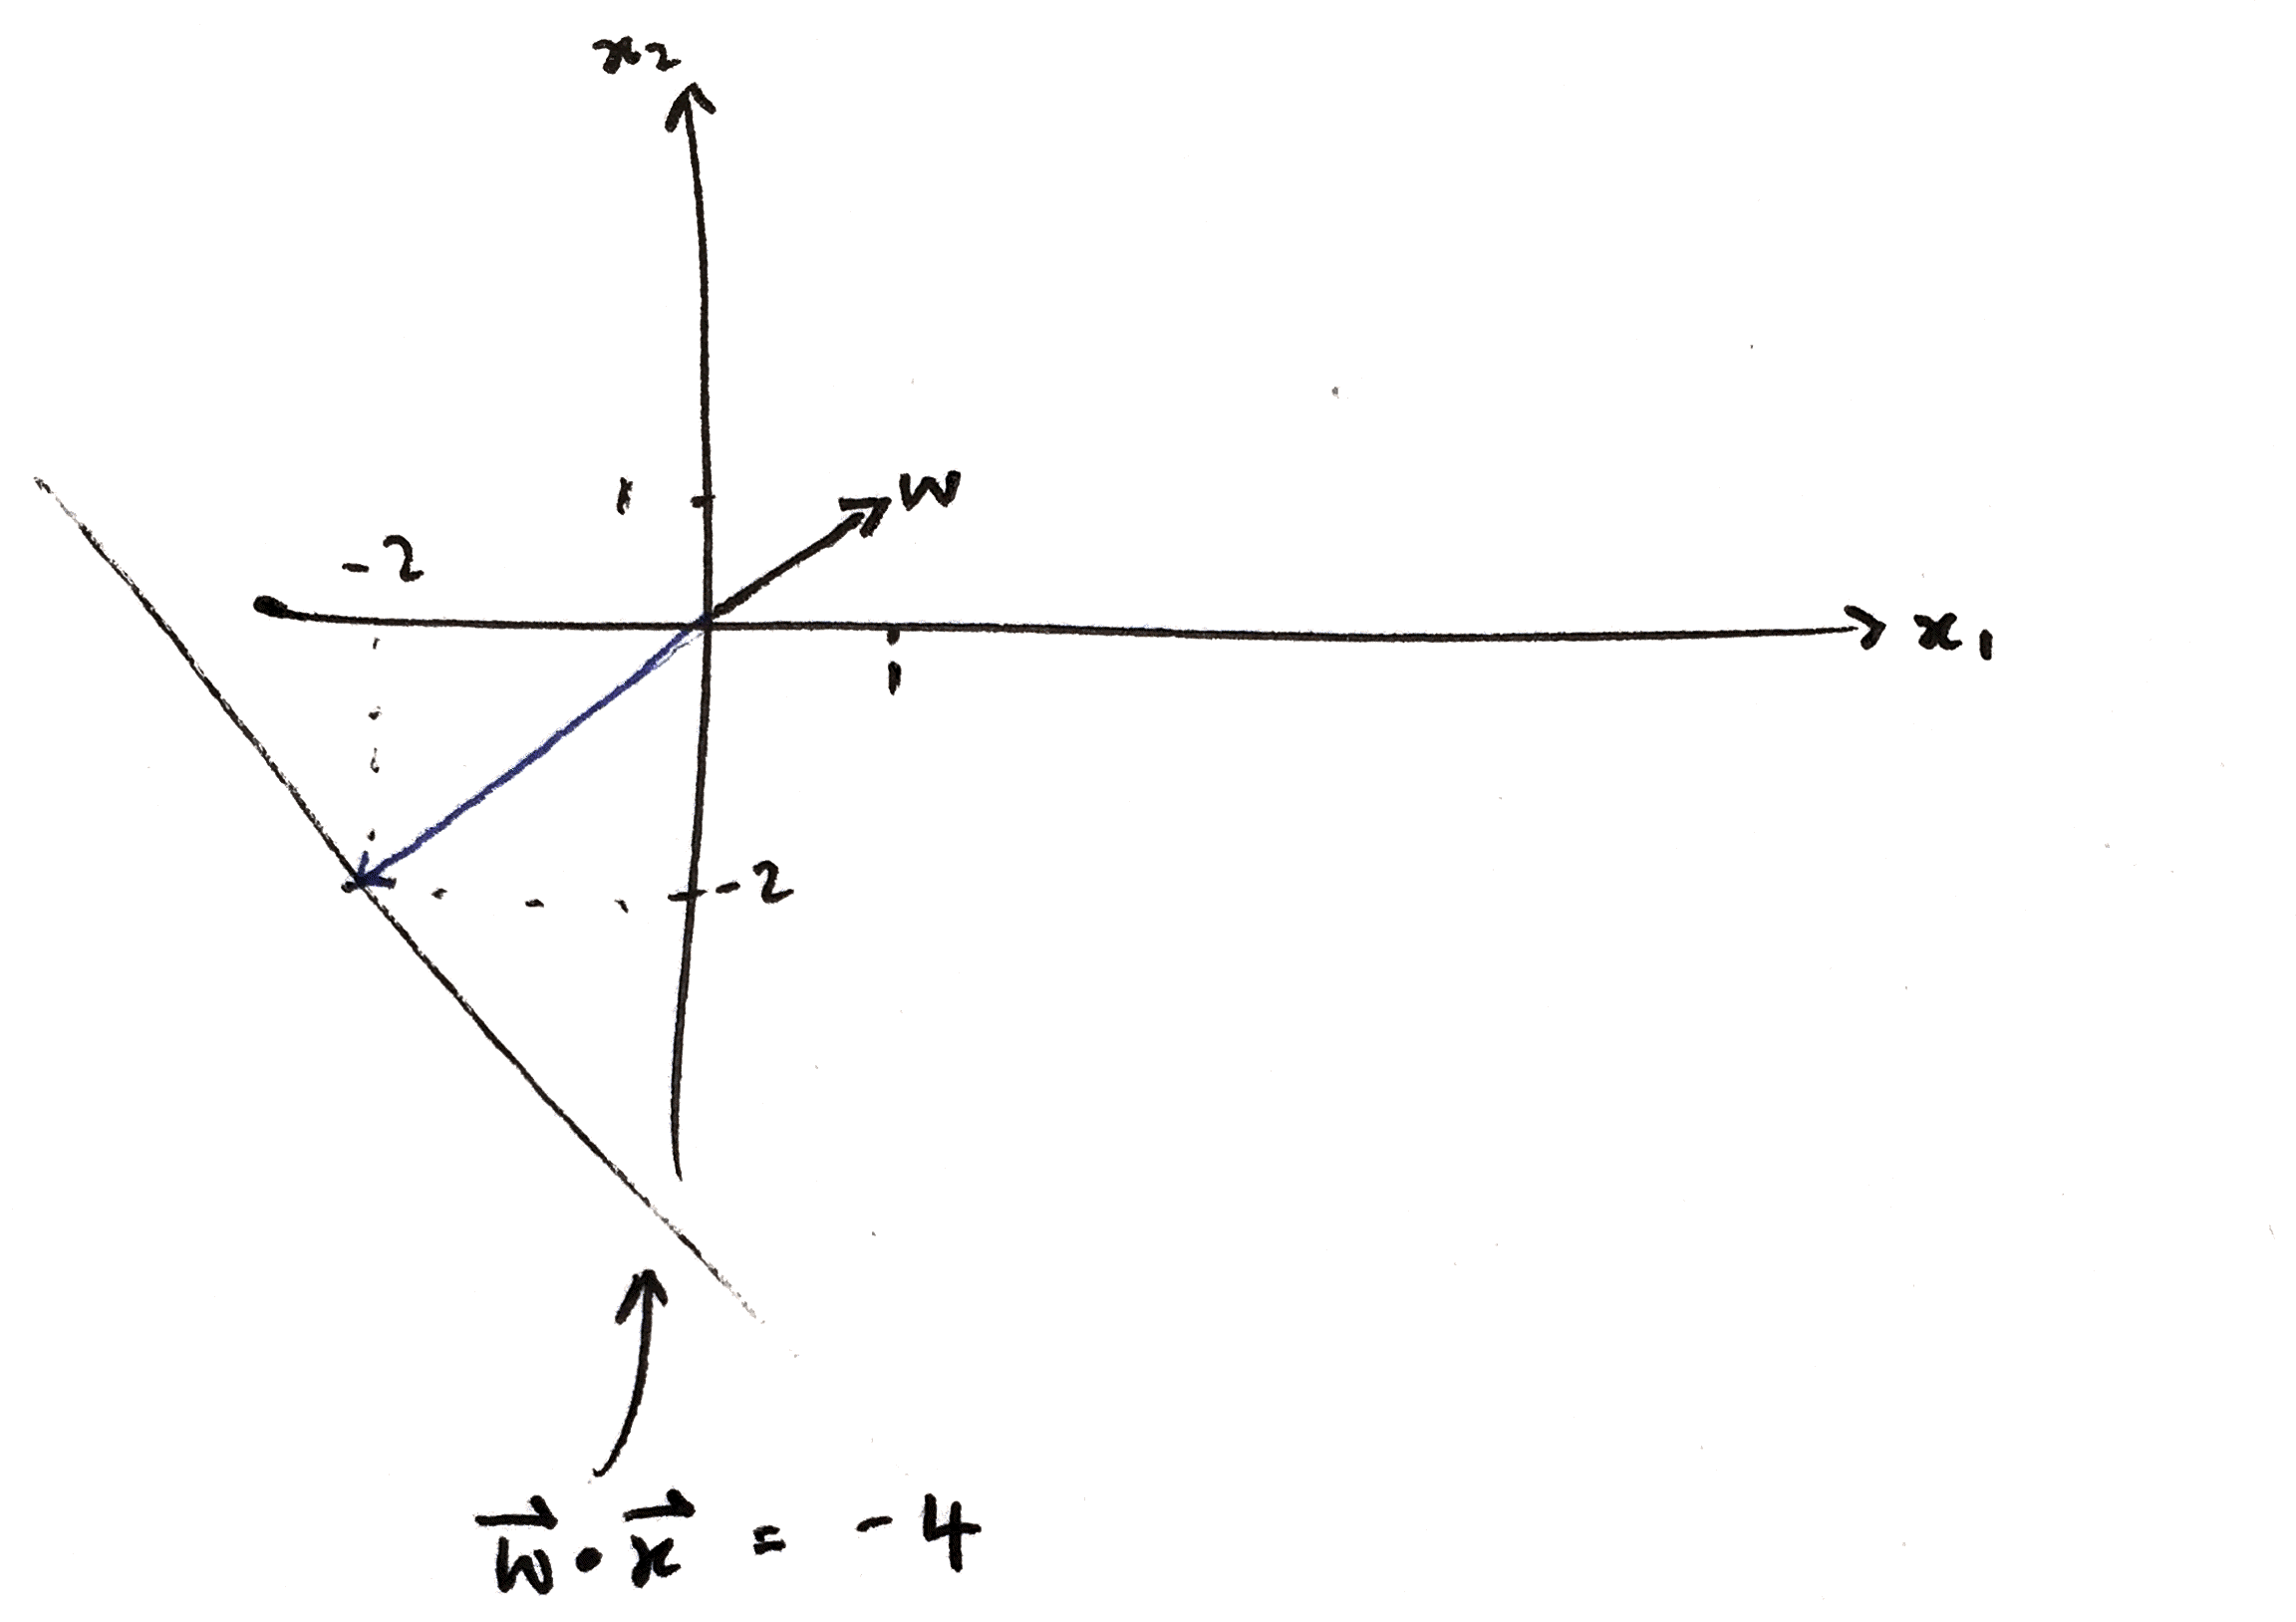
\includegraphics[width=200pt]{img/machine-learning-linear-decision-boundary.png}
\begin{itemize}
\item A plane sloping up at 45° in the north-east direction.
\item Each input feature has equal influence on the classification.
\item Decision boundary is line $x_1 + x_2 = -4$.
\item $\w$ is normal to the decision boundary since $\w \cdot (\x_1 - \x_2) = -4 - (-4) = 0$.
\item If one feature has a very high weight then $\w$ points close to that
  axis and the decision boundary is almost perpendicular to that axis (other
  features almost don't matter).
\end{itemize}

\textbf{Distance from the decision boundary to a point}: For some point $\x_i$,
the height of the decision function plane above $\x_i$ is
$\w \cdot \x_i + \alpha$. At the decision boundary, this height is
zero. Looking ``straight up'' the slope of the decision function, its gradient
is $\sqrt{w_1^2 + w_2^2} = |\w|$. So the distance of a point $\x_i$ from the
hyperplane is $\frac{\w \cdot \x_i + \alpha}{|\w|}$. If $\w$ is not a unit
vector, the problem can be rescaled so that it is, in which case the distance
is $\w \cdot \x_i + \alpha$.
\\
% \begin{mdframed}
%   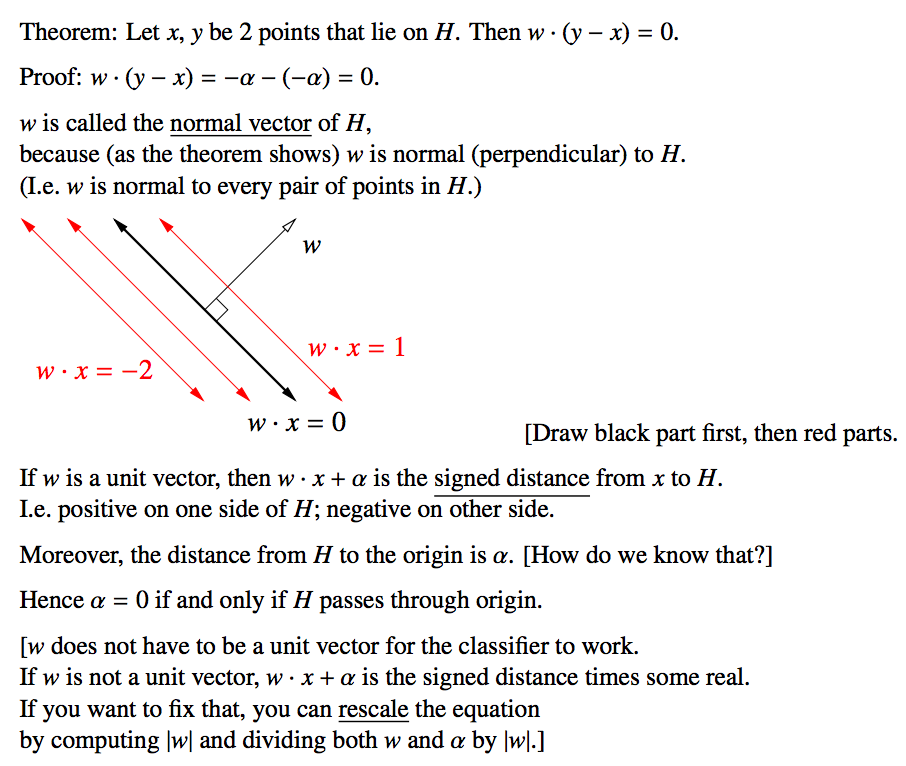
\includegraphics[width=300pt]{img/machine-learning-linear-decision-boundary-2.png}
% \end{mdframed}

\textbf{Examples of linear classifiers}:
\begin{itemize}
\item \textbf{Centroid method}:  Decision boundary perpendicular to and bisects line
  connecting means of labeled training points.
\item \textbf{Perceptron}:
\item \textbf{Maximum margin classifier}:
\item \textbf{LDA}:  Fit Gaussians to each class, same covariance across classes.
\end{itemize}

\subsection*{Perceptron}

Labels $y_i \in \{-1, 1\}$. Assume $\alpha=0$ for now (decision boundary through origin).

\textbf{Goal}: find line separating points (separating hyperplane). I.e. Find $\w$ such that
\begin{align*}
  \begin{cases}
    \x_i \cdot \w \leq 0, &y_i = -1 \\
    \x_i \cdot \w \geq 0, &y_i = +1.
  \end{cases}
\end{align*}
This is equivalent to the \textbf{constraint} $y_i\x_i \cdot \w \geq 0$.

\textbf{Cost function}: total distance $R(\w)$ of misclassified points from the
decision boundary.
\\
\begin{mdframed}
  \textbf{Optimization problem}: Find $\w$ that minimizes
  \begin{align*}
    R(w) = \sum_i L(\x_i \cdot \w, y_i) = \sum_{i \in V} -y_i\x_i \cdot \w,
  \end{align*}
  where $V$ are the misclassified points.
\end{mdframed}

Per-training point loss function
\begin{align*}
  L(\text{prediction}_i, y_i) = L(\x_i \cdot \w, y_i) =
  \begin{cases}
    0, &\text{correct}, y_i\x_i \cdot \w \geq 0\\
    -y_i\x_i \cdot \w, &\text{misclassified}
  \end{cases}
\end{align*}


\textbf{Gradient descent}: Find $w$ that minimizes $R(w)$.


\begin{align*}
  \nabla_w R = \cveccc{-\sum_i y_iX_{i1}}
                      {\vdots}
                      {-\sum_i y_iX_{id}}
\end{align*}
\begin{itemize}
\item On each iteration, compute the gradient; update $\w$ by taking a step
  downhill of size $\rho$: $\w \leftarrow \w + \rho \sum_{i \in V} y_i\x_i$.
\item A misclassified data point far out in dimension $j$ will cause the
  gradient to have a large component $-\sum_i y_iX_{ij}$ in that dimension.
\item $\w$ thus becomes more closely aligned with that axis and the decision
  boundary.
\item Decision boundary therefore becomes more perpendicular to that axis (axis
  becomes more ``important'').
\end{itemize}

\textbf{Stochastic gradient descent (Perceptron)}: on each iteration pick one misclassified
point and update $\w$ using gradient for that point:
$\w \leftarrow \w + \rho y_{i^*}\x_{i^*}$

\textbf{Allow decision boundaries that do not pass through origin}: add a
fictitious dimension so that sample points now lie on the plane $x_{d+1} = 1$
in $(d+1)$ dimensions. Run algorithm as above, just with the new
dimensionality.
\begin{align*}
  \w \cdot \x + \alpha &= 0 \\
  \cveccc{w_1}
         {w_2}
         {\alpha} \cdot \cveccc{x_1}{x_2}{1} &= 0.
\end{align*}

\subsection*{Optimization in weight space}

\begin{tabular}{l|l}
  $\x$-space    & $\w$-space \\
  \hline
  hyperplane & point $\w$ is normal vector to hyperplane \\
  point      & hyperplane whose normal vector is the $\x$ point (? don't understand this yet)
\end{tabular}

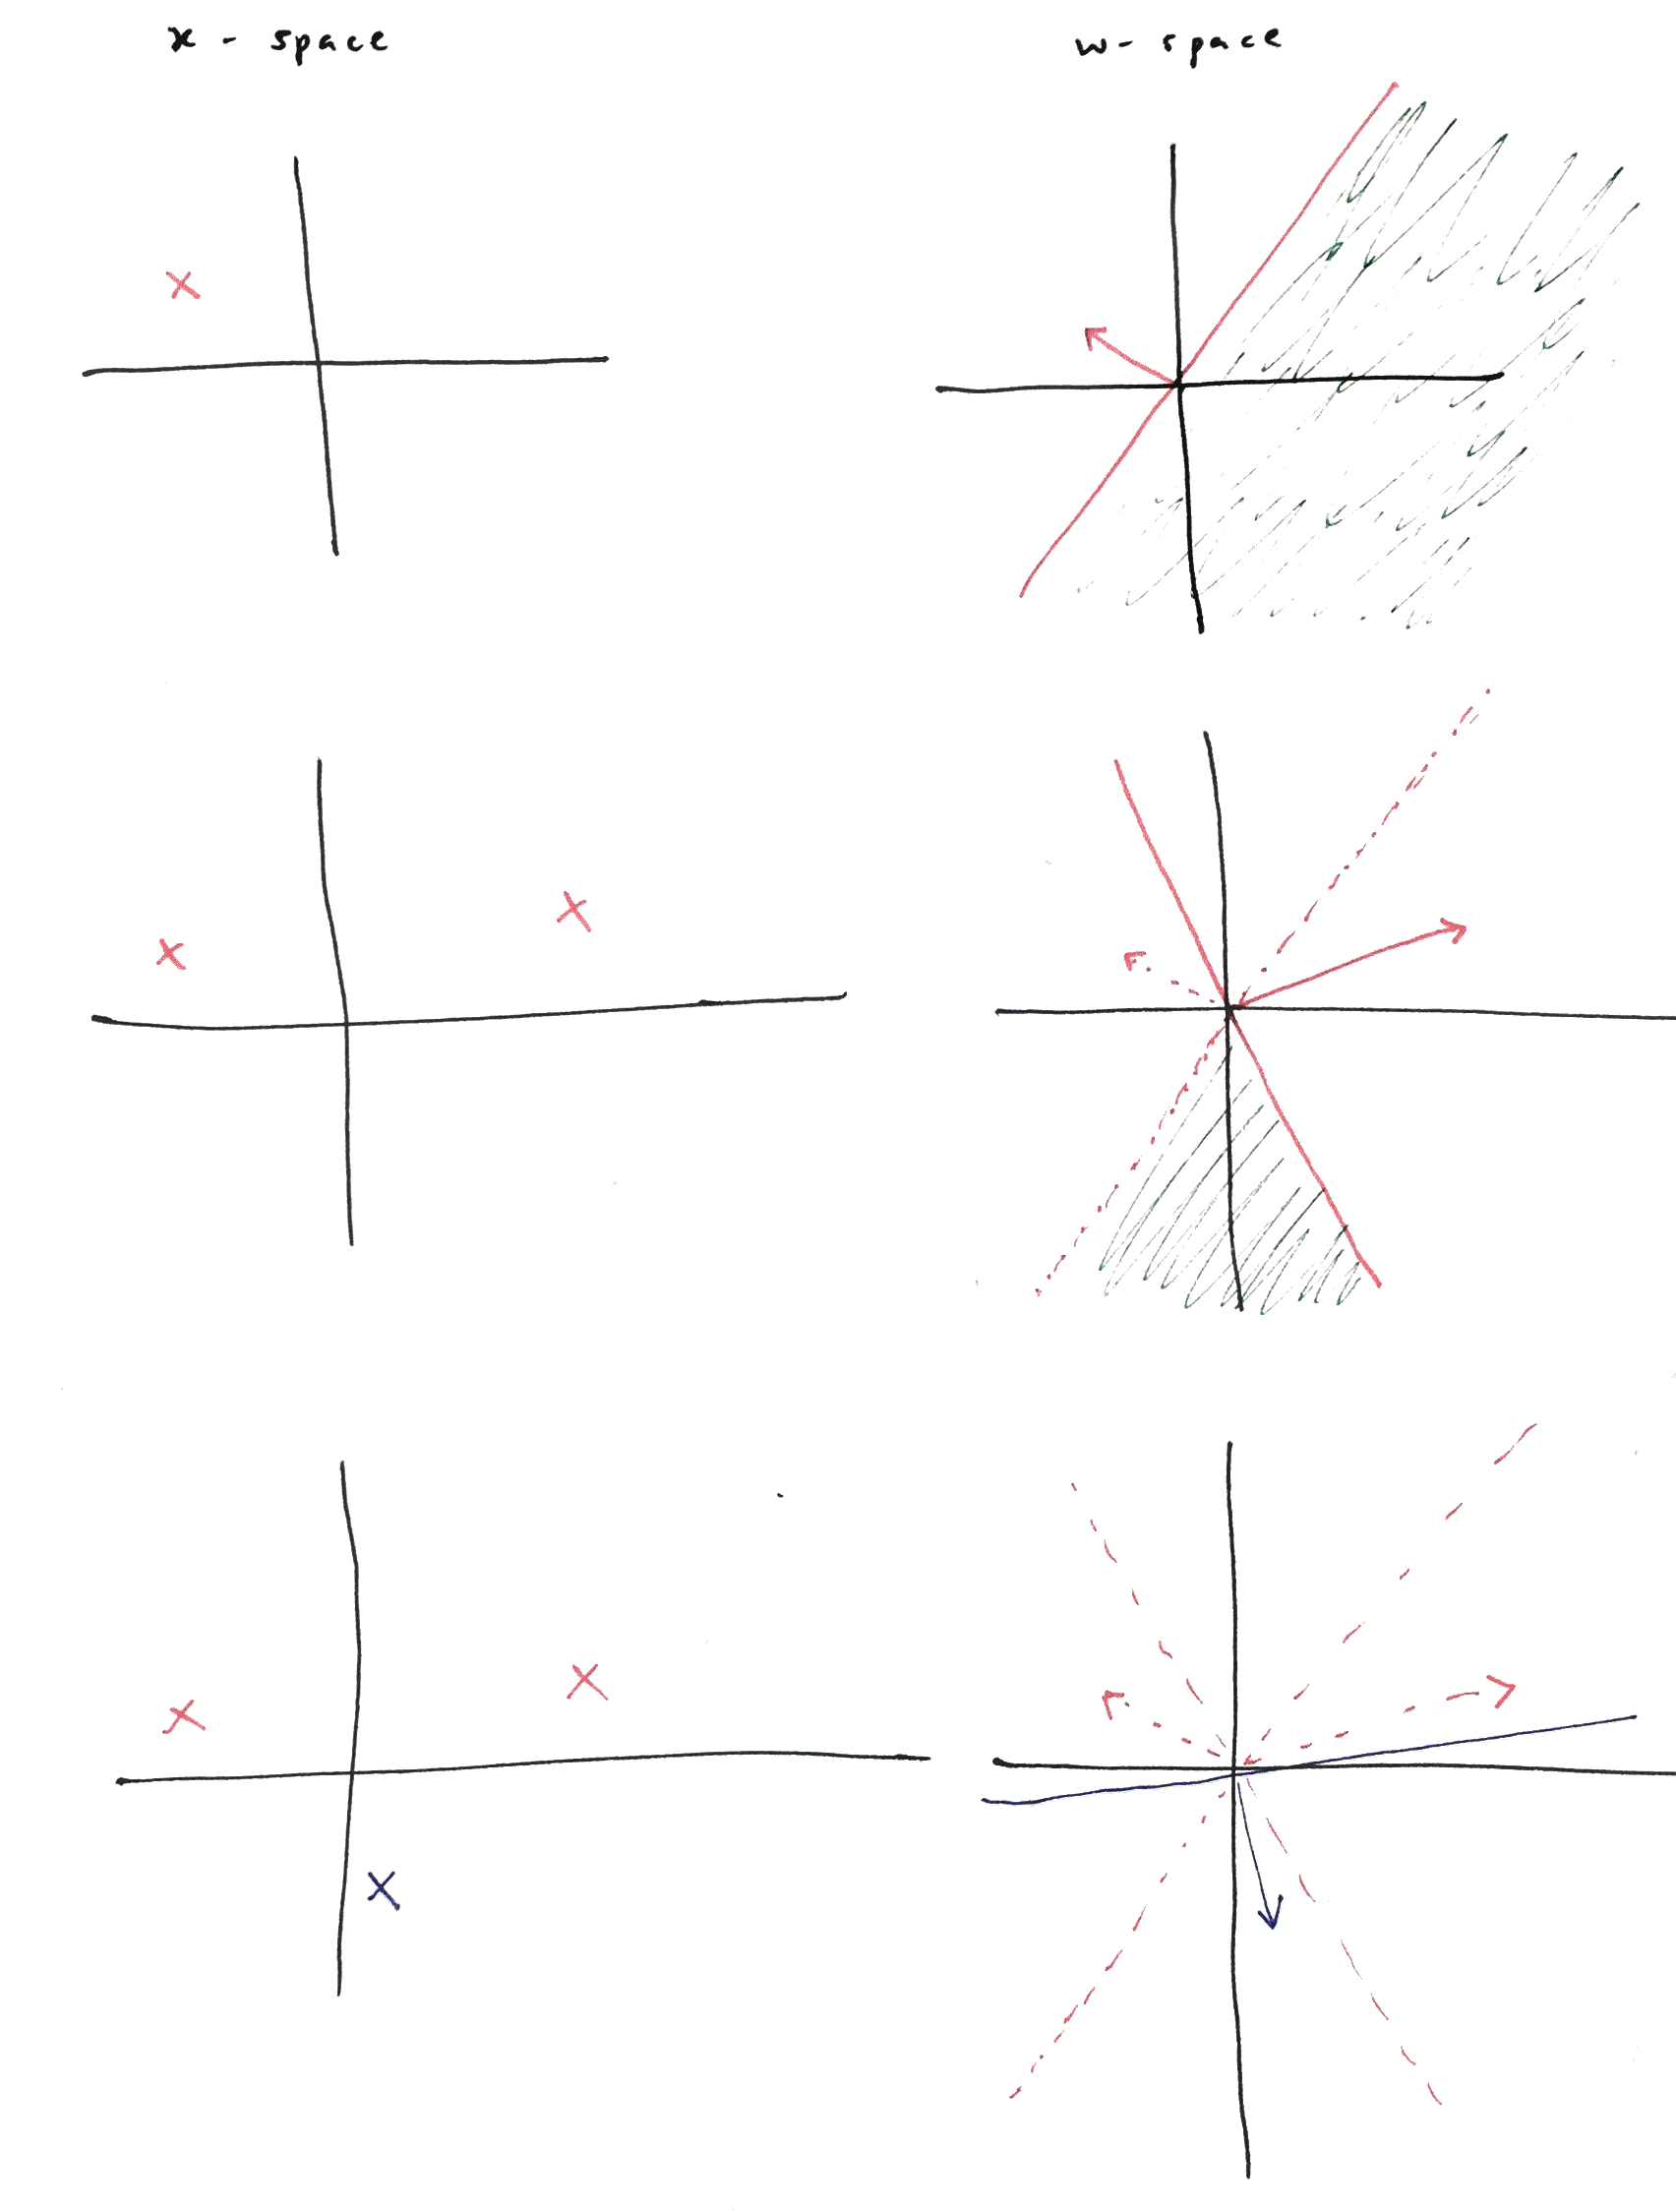
\includegraphics[width=200pt]{img/ml-perceptron-x-space-w-space.png}

\subsection*{Maximum margin classifiers}
\textbf{Margin} is distance from hyperplane to nearest sample point.

Previously, in the perceptron, we used the constraint
$$y_i \x_i \cdot \w \geq 0.$$
Now, we demand that there is a non-zero margin between the decision boundary
and the points:
$$y_i (\x_i \cdot \w + \alpha) \geq 1,$$
The 1 on the RHS is arbitrary; I think $\w$ and $\alpha$ will adapt to make it
true for any positive value, so the point is that we're demanding a strictly
non-zero margin.
\\
\begin{mdframed}
  \textbf{Optimization problem (quadratic program)}:\\
    Find $\w, \alpha$ that minimize $|\w|^2$ such that
    $y_i(\x_i \cdot \w + \alpha) \geq 1$ for all points $i$.
\end{mdframed}

\subsection*{Soft margin SVMs}

\begin{itemize}
\item Still quadratic program but allow points to violate margin via
  \textbf{slack variables} $\xi_i$:
\item Constraint is $y_i(\x_i \cdot \w + \alpha) \geq 1 - \xi_i$
\item Find non-linear decision boundaries by introducing new features
  comprising non-linear functions of base features (``lift points into
  higher-dimensional space'').
\end{itemize}

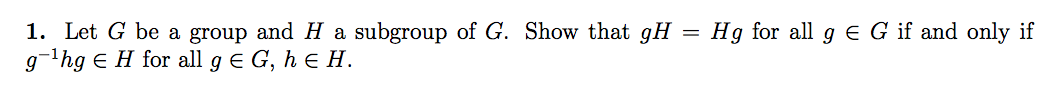
\includegraphics[width=300pt]{img/ml-svm-parabolic-lifting.png}

TODO\\
\url{https://people.eecs.berkeley.edu/~jrs/189/lec/04.pdf}\\
\url{https://www.youtube.com/watch?v=HOZ6ZpPA_Ks}

\section*{5 Machine Learning Abstractions and Numerical Optimization}
TODO\\
\url{https://people.eecs.berkeley.edu/~jrs/189/lec/05.pdf}\\
\url{https://www.youtube.com/watch?v=DeIAXPUfCbQ}

\section*{6 Decision Theory; Generative and Discriminative Models}
https://people.eecs.berkeley.edu/~jrs/189/lec/06.pdf
https://www.youtube.com/watch?v=aXkenQ01qYI

\section*{7 Gaussian discriminant analysis}
https://people.eecs.berkeley.edu/~jrs/189/lec/07.pdf
https://www.youtube.com/watch?v=4CefboCXxZs

\section*{8 Eigenvectors and the Anisotropic Multivariate Gaussian Distribution}
https://people.eecs.berkeley.edu/~jrs/189/lec/08.pdf

\section*{9 The Anisotropic Multivariate Normal Distribution, QDA, and LDA}

\section*{10 Regression, including Least-Squares Linear and Logistic Regression}
\newpage
\subsection*{Linear Least Squares Regression}
Use fictitious dimension trick, so that $\w$ includes the offset term and $\X$
is $(n \times (d + 1))$.
\\
\begin{mdframed}
Find $\w$ that minimizes cost function $J(w)$: sum of squared difference between
linear predictor and observed training point.
\begin{align*}
  J(w) = |\X \w - \y|^2 = \sum_i (\x_i^\T\w - y_i)^2
\end{align*}
\end{mdframed}

Solve by differentiating and finding the critical point:
\begin{align*}
  |\X \w - \y|^2          &= \w\X^\T\X\w - 2\y^\T\X\w + \y^\T\y \\
  \grad_\w |\X \w - \y|^2 &= 2 \X^\T\X\w - 2\X^\T\y \\
  \w^*                    &= (\X^\T\X)^{-1}\X^\T\y =: \X^+\y
\end{align*}
\begin{mdframed}
For a new sample point $\x$, the prediction is $\hat y = \x \cdot \w^*$.
\end{mdframed}

\subsubsection*{Related concepts}
\begin{itemize}
\item \textbf{normal equations}: linear system of $d$ equations in unknown $\w$ resulting from
  setting the gradient equal to zero: $\X^\T\X\w - \X^\T\y = \vec 0$
\item \textbf{pseudoinverse}: The matrix $\X^+ = (\X^\T\X)^{-1}\X^\T$ maps $\y$
  to $\w^*$. In general there's no $\w$ that solves $\X\w = \y$, but
  $\w^* = \X^+\y$ makes the LHS as close as possible to $\y$. So it behaves as
  a ``left inverse'' of $\X$, since $\X^+\X = \I$ and left-multiplying by $\X^+$
  gives the ``solution'' to $\X\w = \y$.
\item \textbf{projection matrix} or \textbf{hat matrix}: Still focusing on the
  training phase, the predictions are $\hat \y = \X\w^* = \X\X^+\y$. So
  $\X\X^+$ puts that hat on $\y$, or projects $\y$ onto the hyperplane, in the
  viewpoint described below.
\end{itemize}

\subsubsection*{Projection interpretation}
Usually we think of $n$ points in $\R^d$. But instead, consider a separate
column of the data for each feature: these are $d$ points in $\R^n$. The
observed training data $\y$ is also a point in $\R^n$, and so is the prediction
$\hat \y = \X\w$.

As we vary $\w$, the prediction $\X\w$ describes a hyperplane spanned by the
columns of $\X$.

We want to find the $\w^*$ corresponding to the closest point on the hyperplane
to $\y$. So $X\w^* - \y$ must be orthogonal to the hyperplane:
\begin{align*}
  \X^\T \cdot (\X\w^* - \y) = \vec 0.
\end{align*}
Which are the normal equations (linear system of $d$ equations), derived
differently.

\subsubsection*{Weighted linear regression}
Sample point $i$ has weight $b_i$. Diagonal $n \by n$ matrix $\mat B$ contains weights.
\begin{align*}
  J(\w) &= \sum_i b_i (\x_i^\T\w - y_i)^2 \\
        & = (\X\w - \y)^\T \B (\X\w - \y) \\
        &= \w^\T\X^\T \B \X\w - 2\y^\T \B \X\w + \y^\T\y
\end{align*}
Gradient
\begin{align*}
  \grad_\w J(\w) = 2\X^\T \B \X\w - 2\X^\T\B\y
\end{align*}
Solution
\begin{align*}
  \w^* = \(\X^\T \B \X\)^{-1}\X^\T\B\y
\end{align*}


\section*{11 More Regression; Newton’s Method; ROC Curves}

\section*{12 Statistical Justifications; the Bias-Variance Decomposition}

\end{document}
